In this section, we examine the differences between quark- and gluon-initiated jets in terms of substructure variables, and to determine to what extent these variables are correlated. Along the way, we provide some theoretical understanding of these observations. The motivation for these studies comes not only from the desire to ``tag'' a jet as originating from a quark or gluon, but also to improve our  understanding of the quark and gluon components of the QCD background relative to boosted resonances.  (\emph{BS: Do we want to mention the MC differences for $q$/$g$ tagging, and that we are more interested in scaling/correlation behaviour rather than absolute tagging rates?})

\subsection{Methodology}

%{\it Start adding outline/discussion of theoretical understanding}
These studies use the $qq$ and $gg$ samples, described previously in Section~\ref{sec:samples}.
Jets are reconstructed using the \antikt algorithm with 
radius parameters of 0.4, 0.8 and 1.2, and have various
jet grooming approaches applied, as described in Section~\ref{sec:substructure}. 
Only leading and subleading jets in each sample are used. 

Figure~\ref{fig:qg_pt500_basics_AKt_R08} shows a comparison of the $\pt$ and $\eta$ distributions of the
 quark and gluon samples with $\pt=500-600$~GeV. 
\begin{figure*}
\begin{center}
\subfigure[Leading jet
\pT]{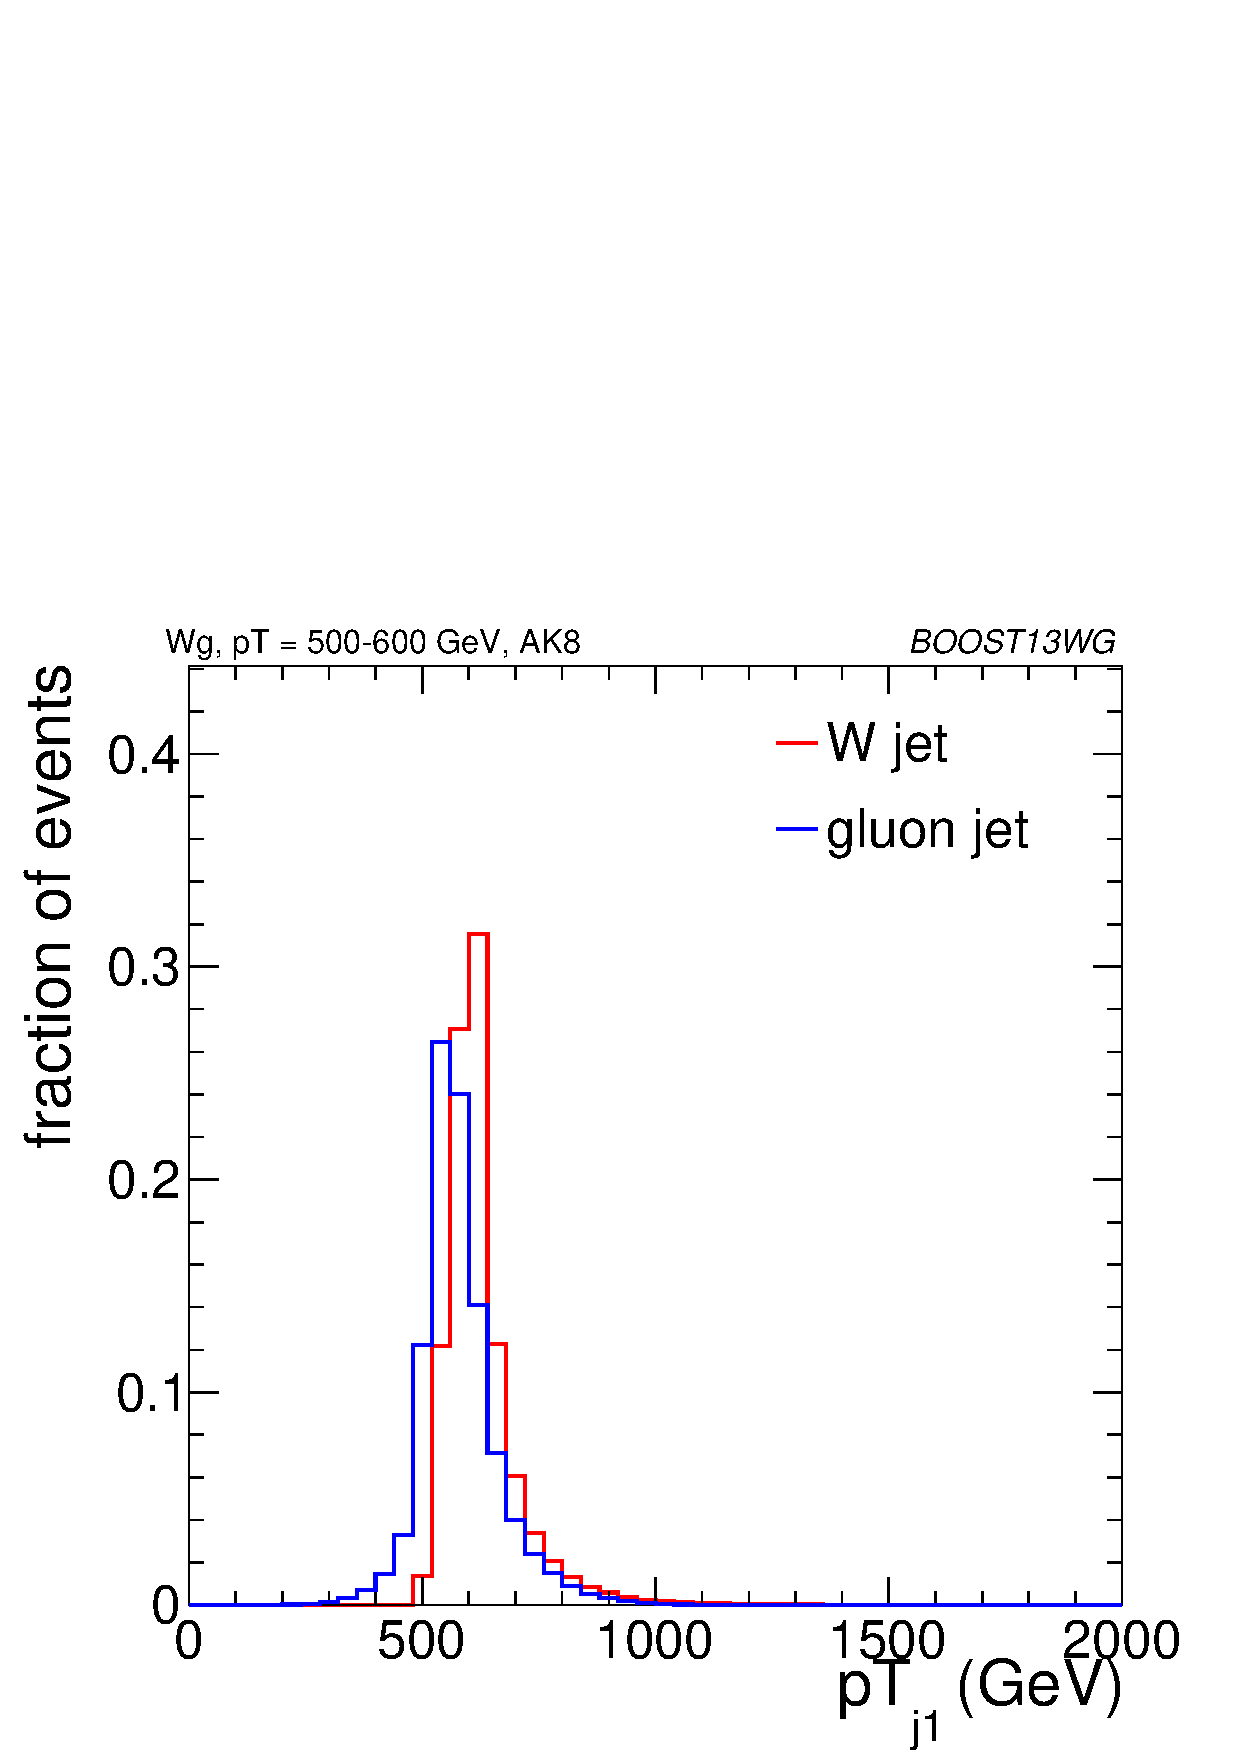
\includegraphics[width=0.40\textwidth]{./Figures/QGTagging/pT500/AKtR08/jpt1.png}}
\subfigure[Sub-leading jet
\pT]{\includegraphics[width=0.40\textwidth]{./Figures/QGTagging/pT500/AKtR08/jpt2.png}}\\
\subfigure[Leading jet
$\eta$]{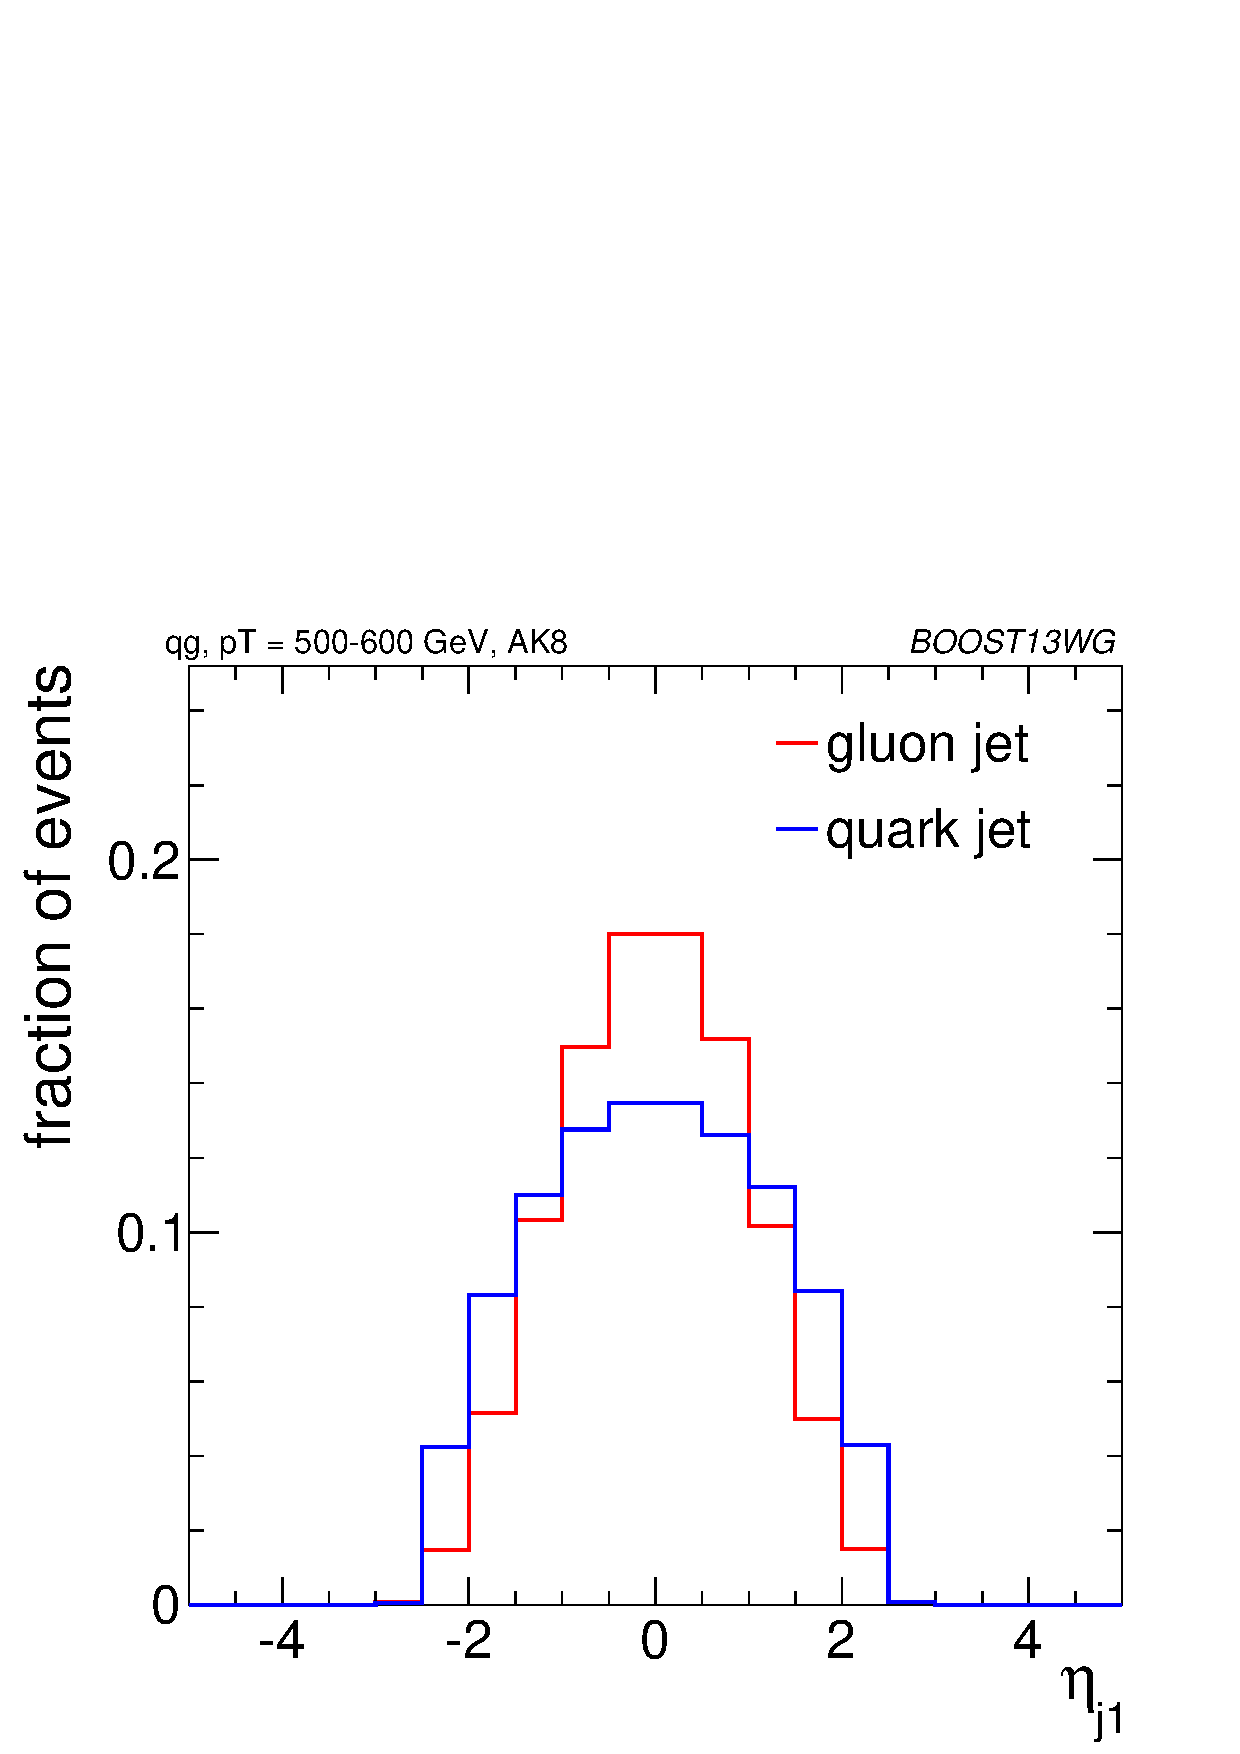
\includegraphics[width=0.40\textwidth]{./Figures/QGTagging/pT500/AKtR08/jeta1.png}}
\subfigure[Sub-leading jet
$\eta$]{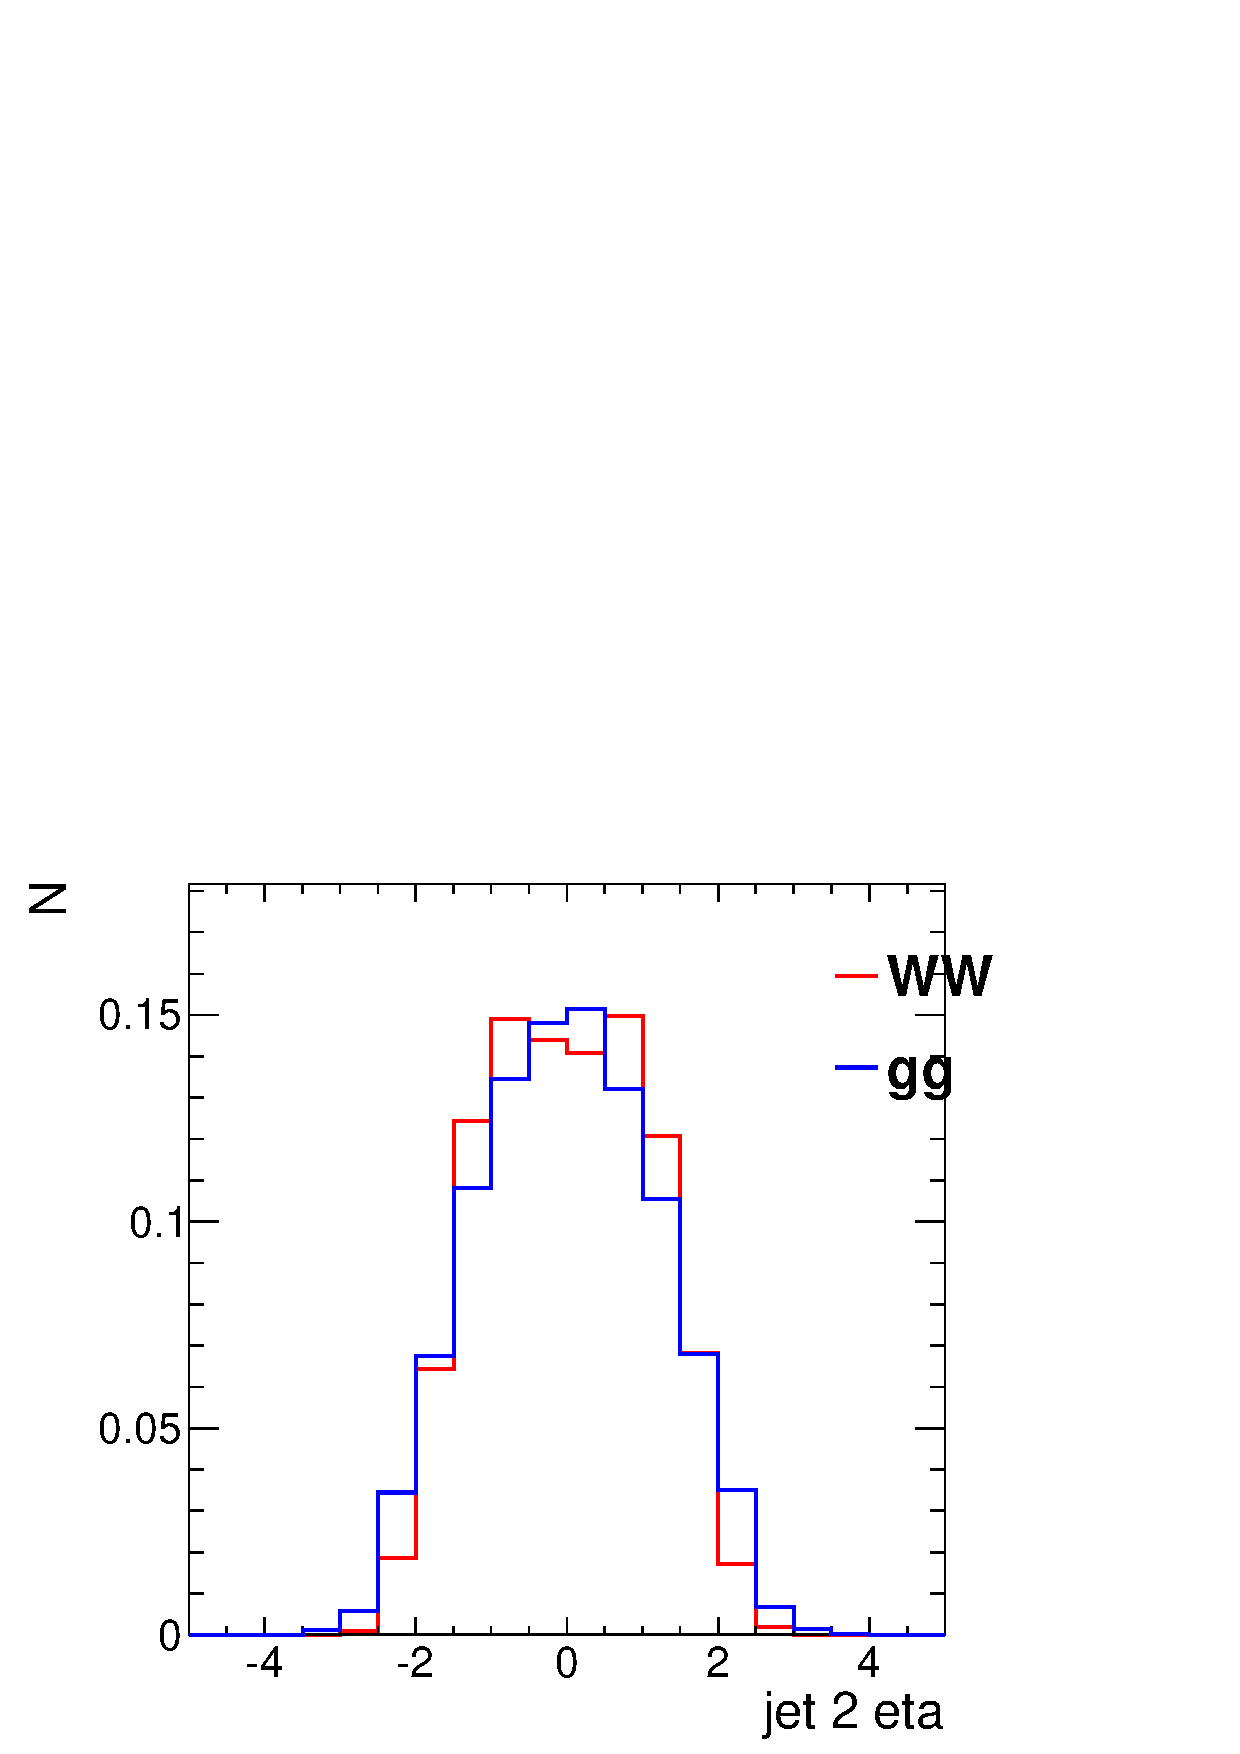
\includegraphics[width=0.40\textwidth]{./Figures/QGTagging/pT500/AKtR08/jeta2.png}}
\caption{Comparisons of quark and gluon $\pt$ and $\eta$ 
distributions in the sample used for the jets of $\pt=500-600 \GeV$ bin using the anti-\kT R=0.8 algorithm.}
\label{fig:qg_pt500_basics_AKt_R08}
\end{center}
\end{figure*}
The differences in the $\pt$ distributions can be attributed to different out-of-cone radiation
patterns for quark and gluons (\emph{BS: Is this just due to an increased likelihood of hard ISR/FSR for $gg$ states due to the larger QCD charge?}), while the different $\eta$ distributions are related to the different
parton distribution functions initiating $qq$ and $gg$ production. The qualitative features of the 
$\eta$ distributions do not change as the $R$ parameter is changed. As the $\pt$ increases, 
the $\eta$ distributions peak more strongly near zero, as expected. Differences in the $\pt$ distributions 
between the leading and sub-leading (and quark and gluon-induced) jets become smaller as the 
$R$ parameter is increased, as expected from the physics behind these differences, outlined above. 

\subsection{Single Variable Discrimination}

(\emph{BS: Do we want to organize this section similar to for top tagging, where we first discuss the performance of each observable at fixed $R$/$\pt$, and then discuss the variations? It's a little mixed right now.})

Figure~\ref{fig:qg_pt500_mass_AKt_R08} shows the mass of jets in the quark and gluon samples when using
different groomers, and Figure~\ref{fig:qg_pt500_subst_AKt_R08} shows similar comparisons for different 
substructure variables. Jets built with the anti-\kT algorithm with R=0.8 and with $\pt=500-650 \GeV$ are used. 
\begin{figure*}
\begin{center}
\subfigure[Ungroomed mass]{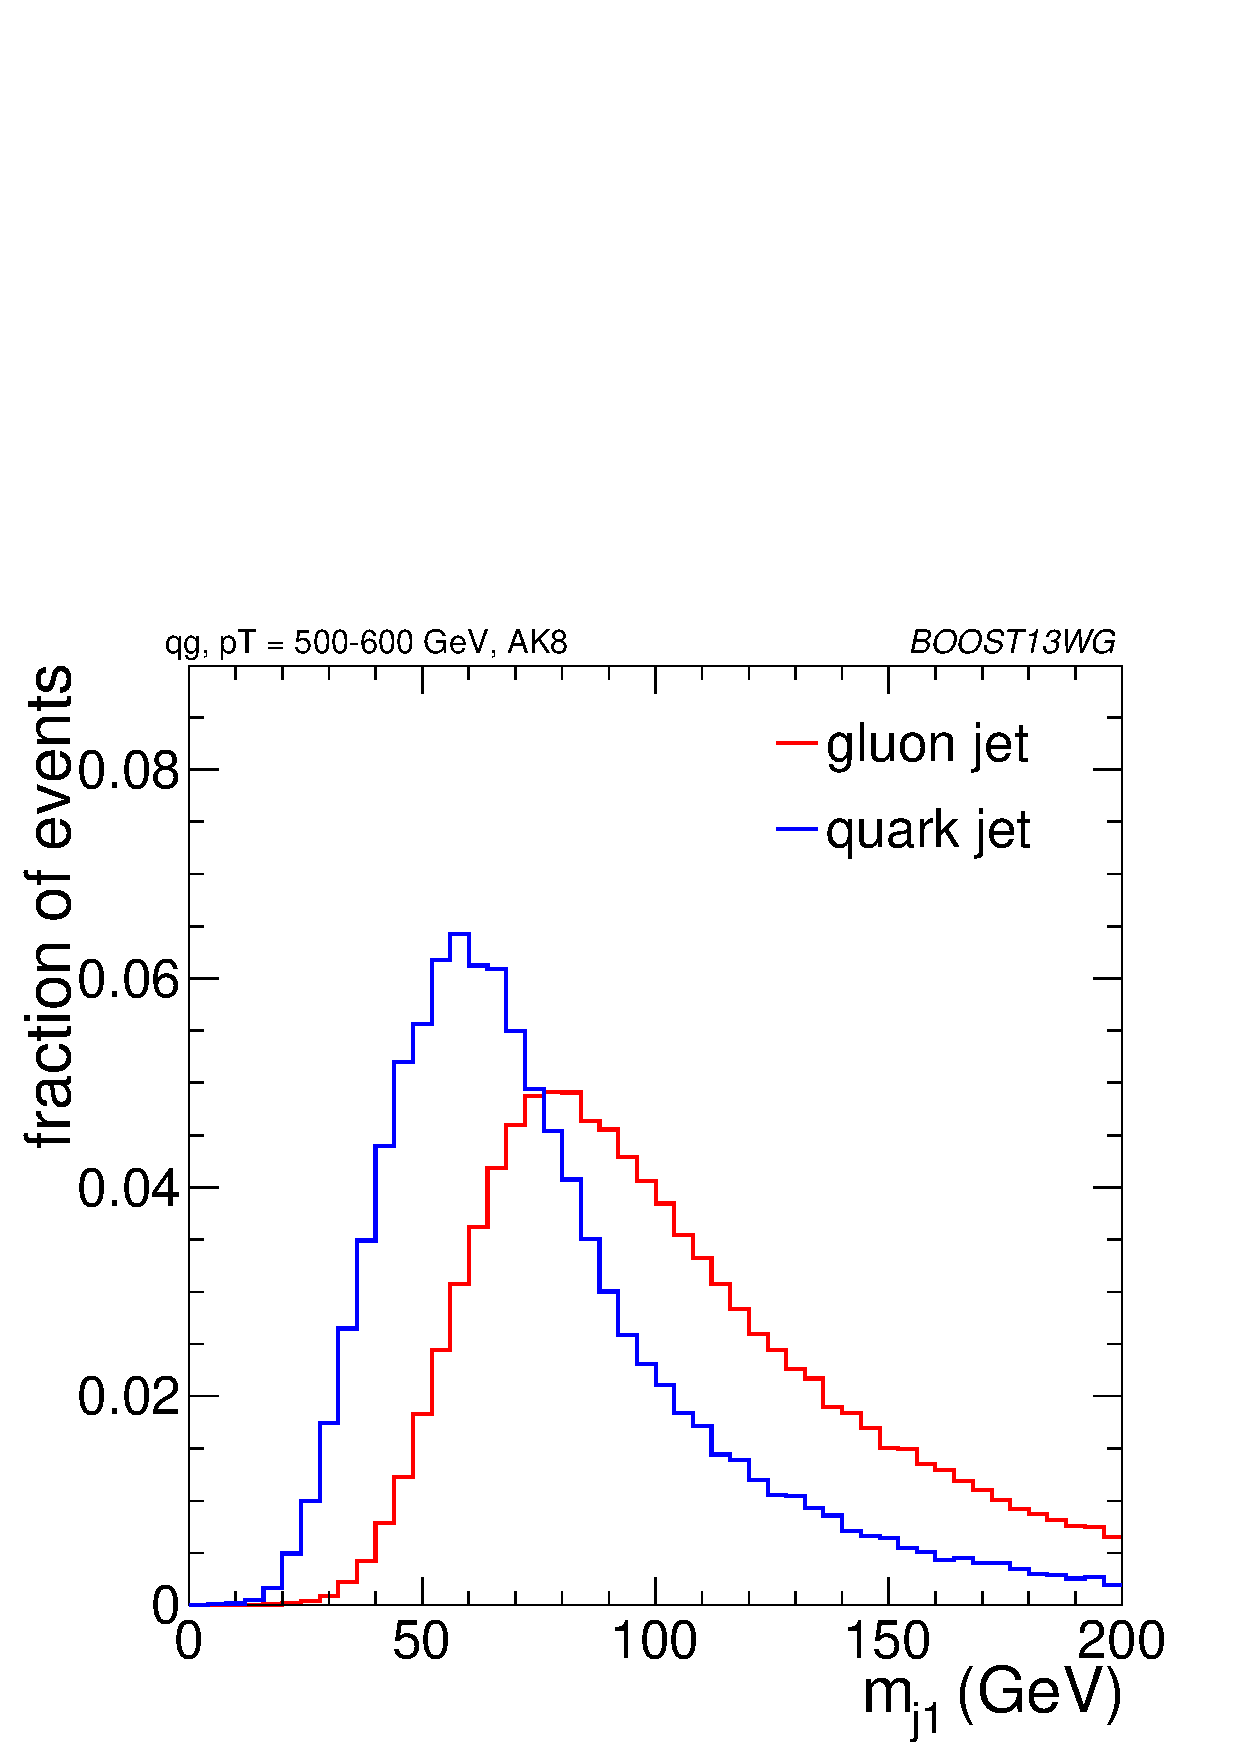
\includegraphics[width=0.30\textwidth]{./Figures/QGTagging/pT500/AKtR08/jmass1.png}}
\subfigure[Pruned mass]{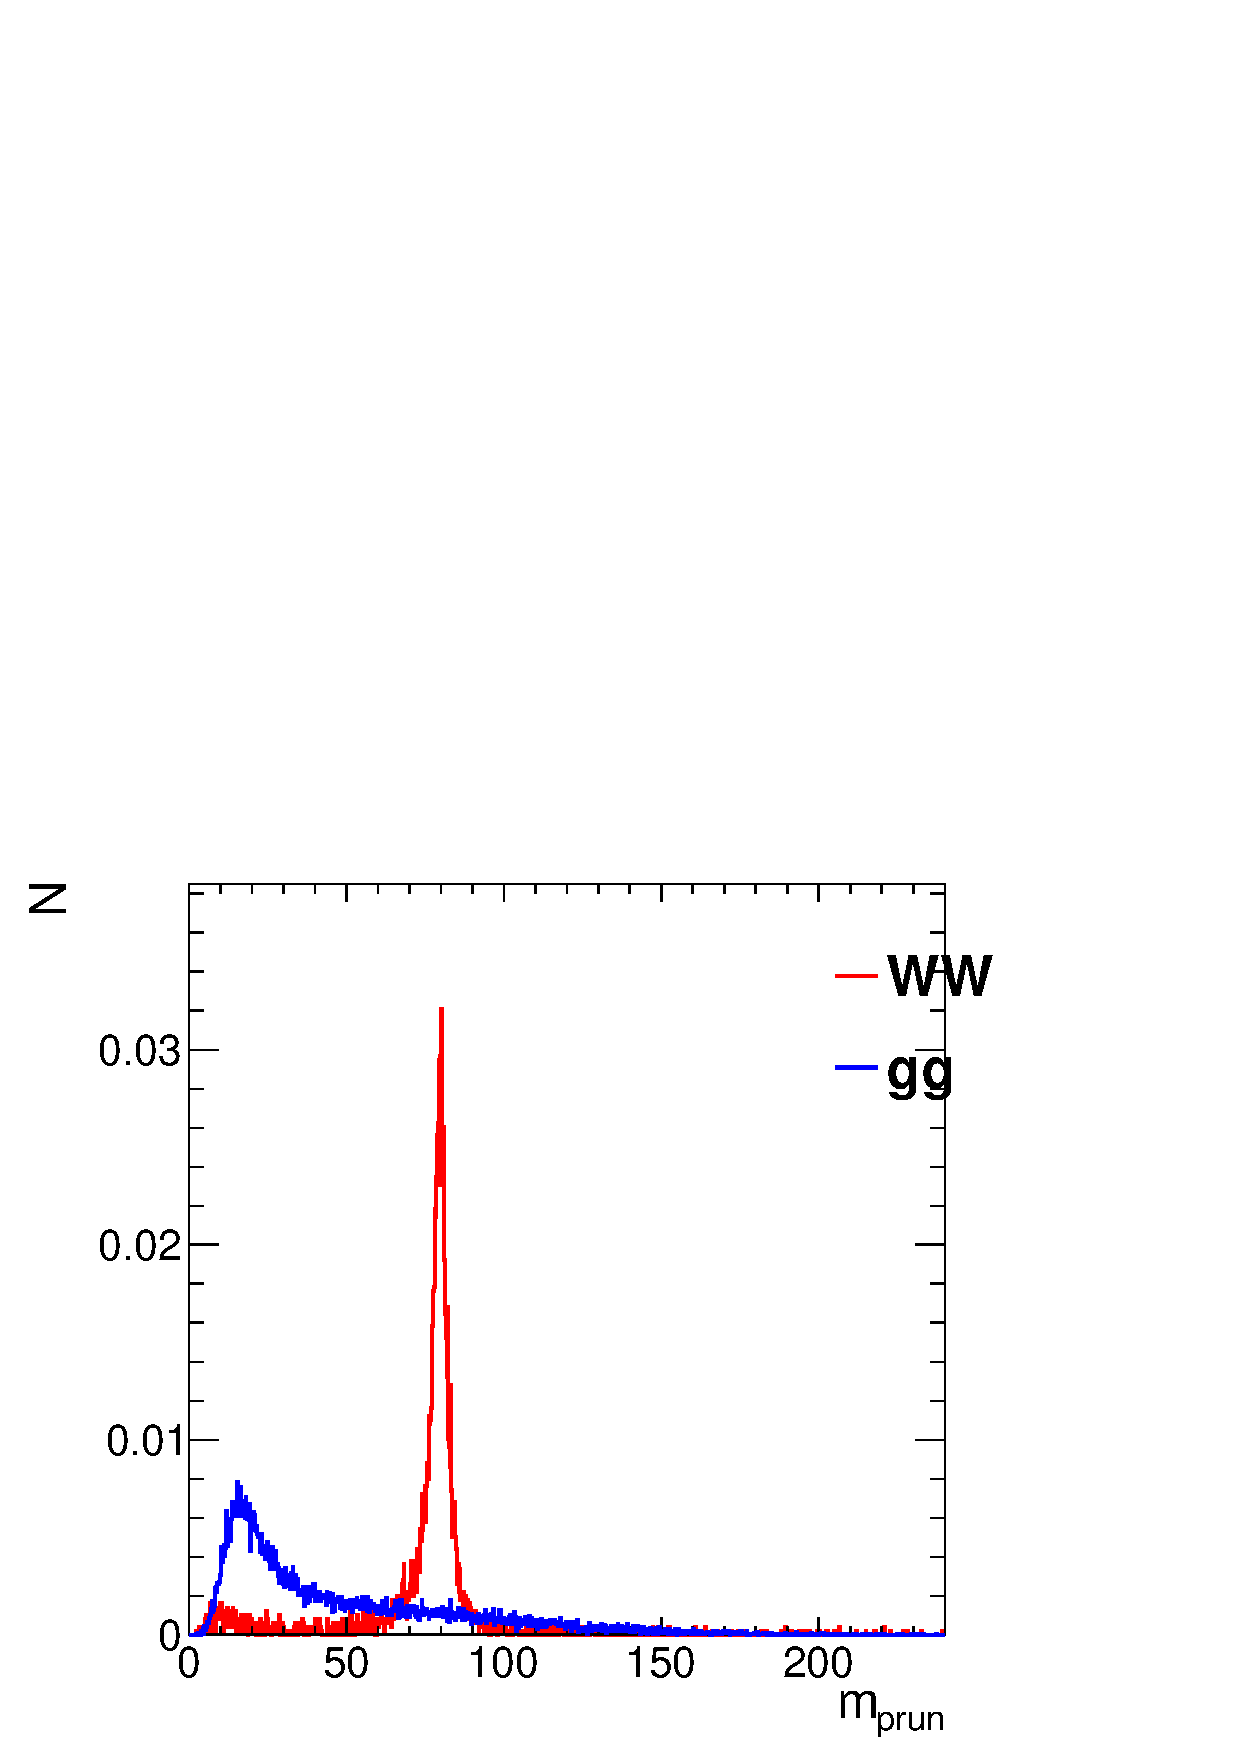
\includegraphics[width=0.30\textwidth]{./Figures/QGTagging/pT500/AKtR08/h_mass_prun.png}}
\subfigure[Trimmed mass]{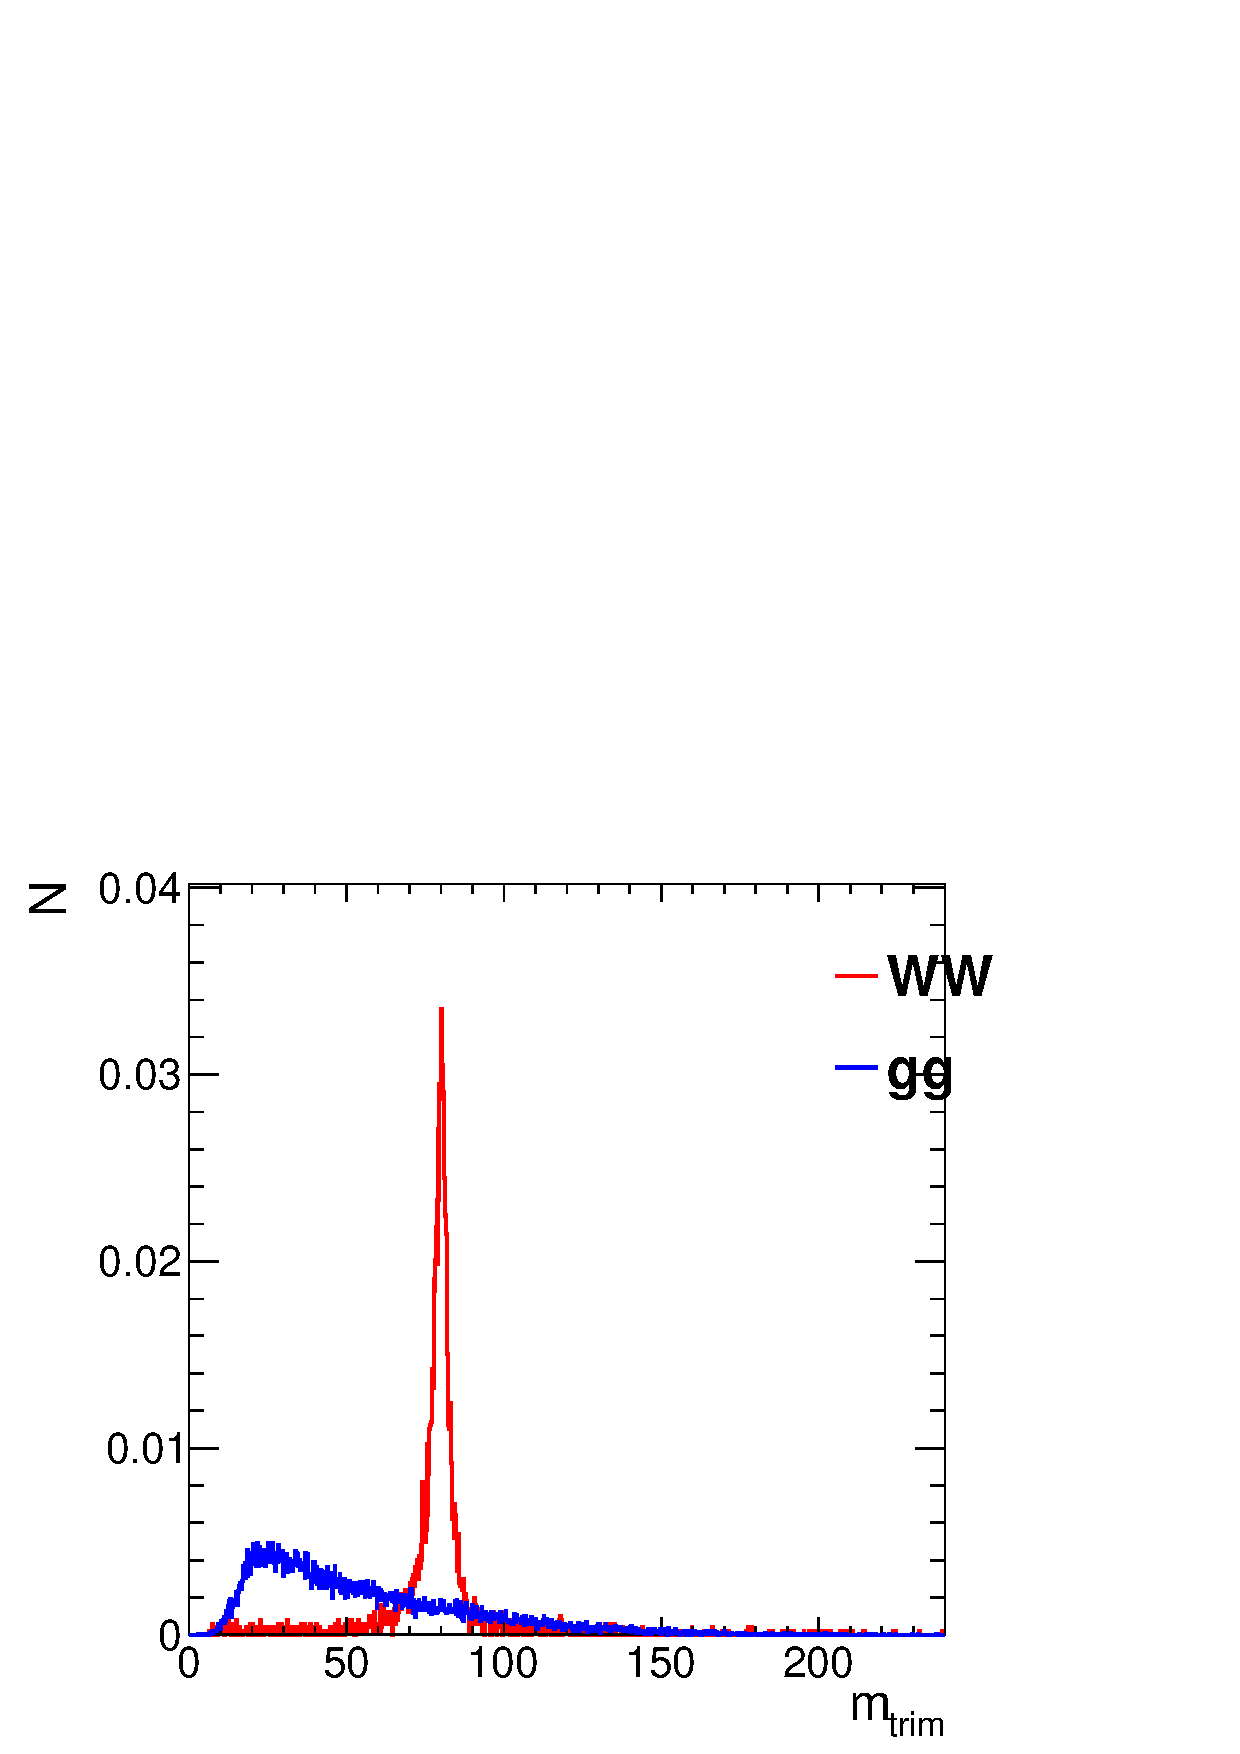
\includegraphics[width=0.30\textwidth]{./Figures/QGTagging/pT500/AKtR08/h_mass_trim.png}}\\
\subfigure[mMDT mass]{\includegraphics[width=0.30\textwidth]{./Figures/QGTagging/pT500/AKtR08/h_mass_mmdt.png}}
\subfigure[Soft-drop $\beta=2$ mass]{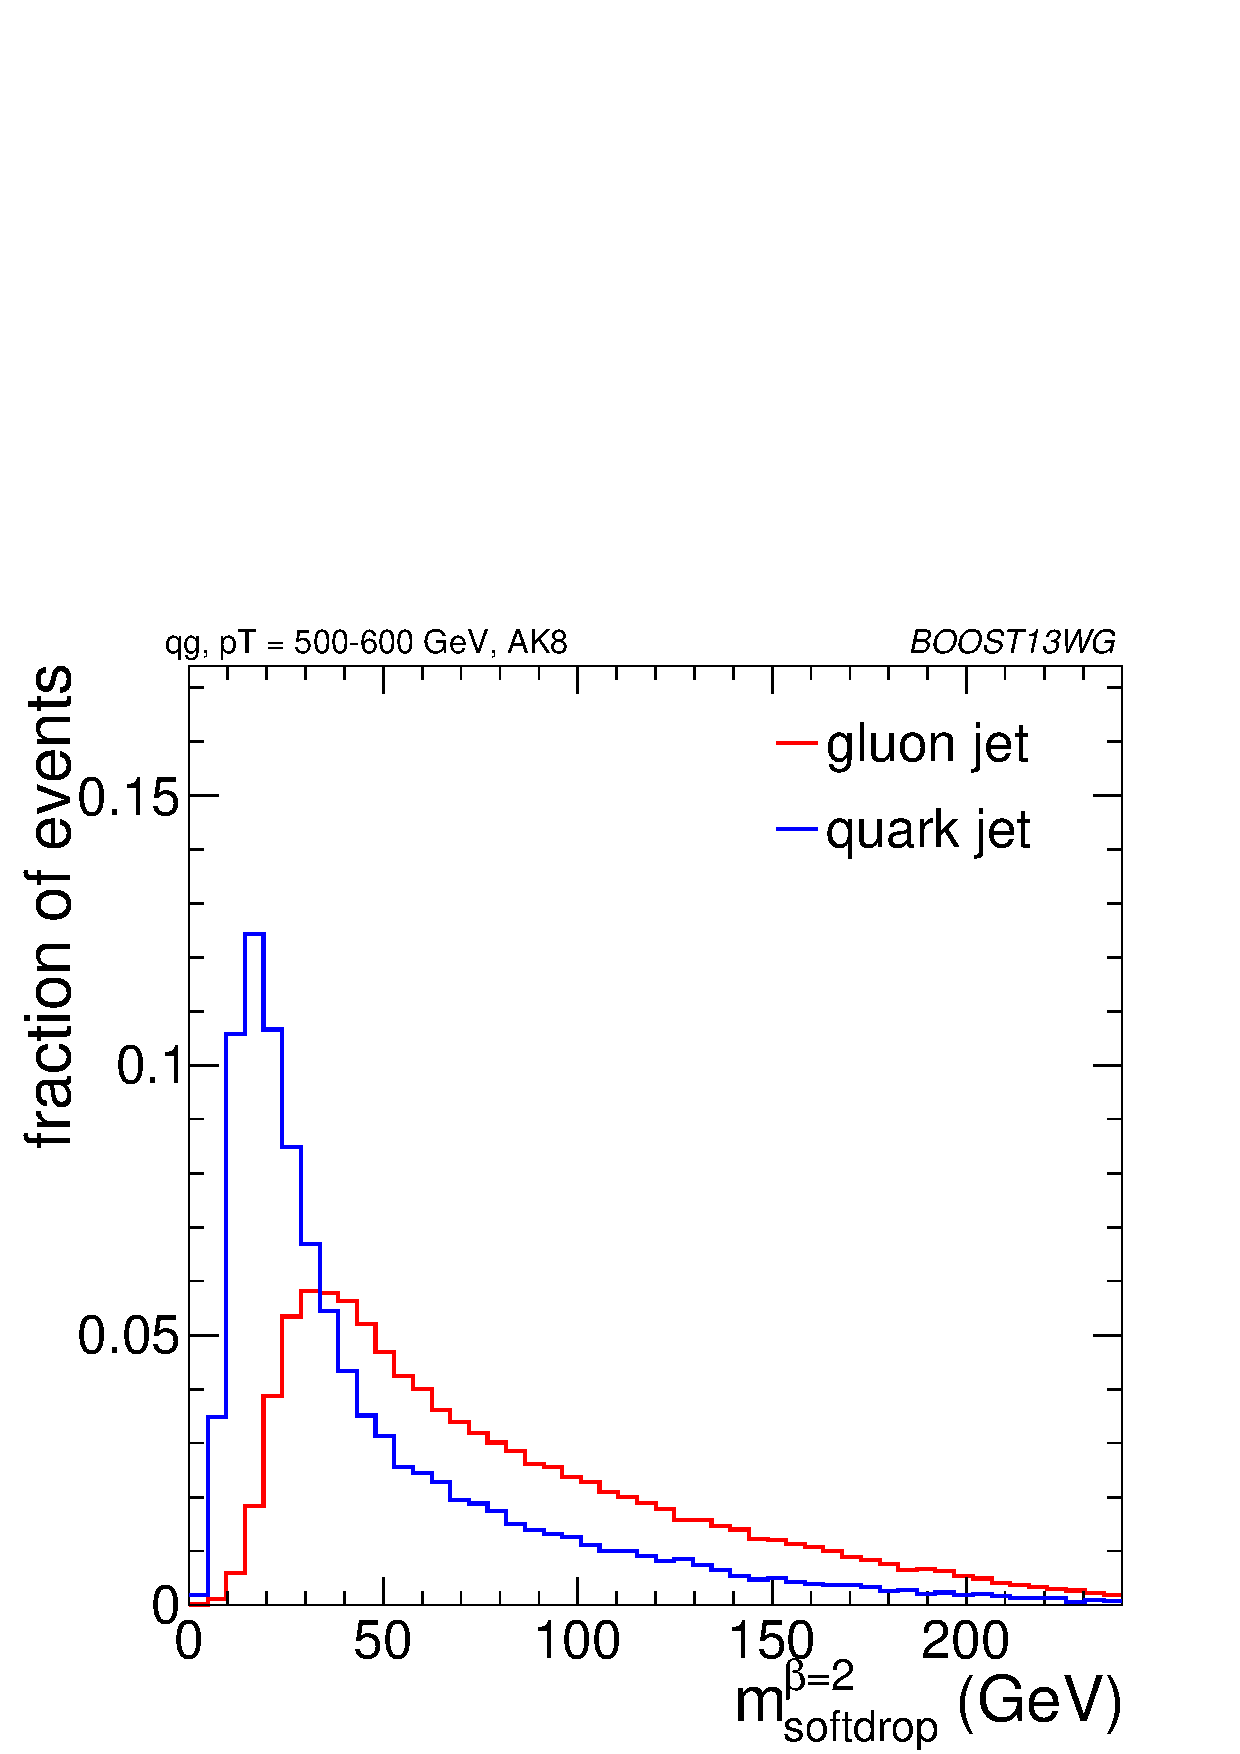
\includegraphics[width=0.30\textwidth]{./Figures/QGTagging/pT500/AKtR08/h_mass_sdb2.png}}
\subfigure[Soft-drop $\beta=-1$ mass]{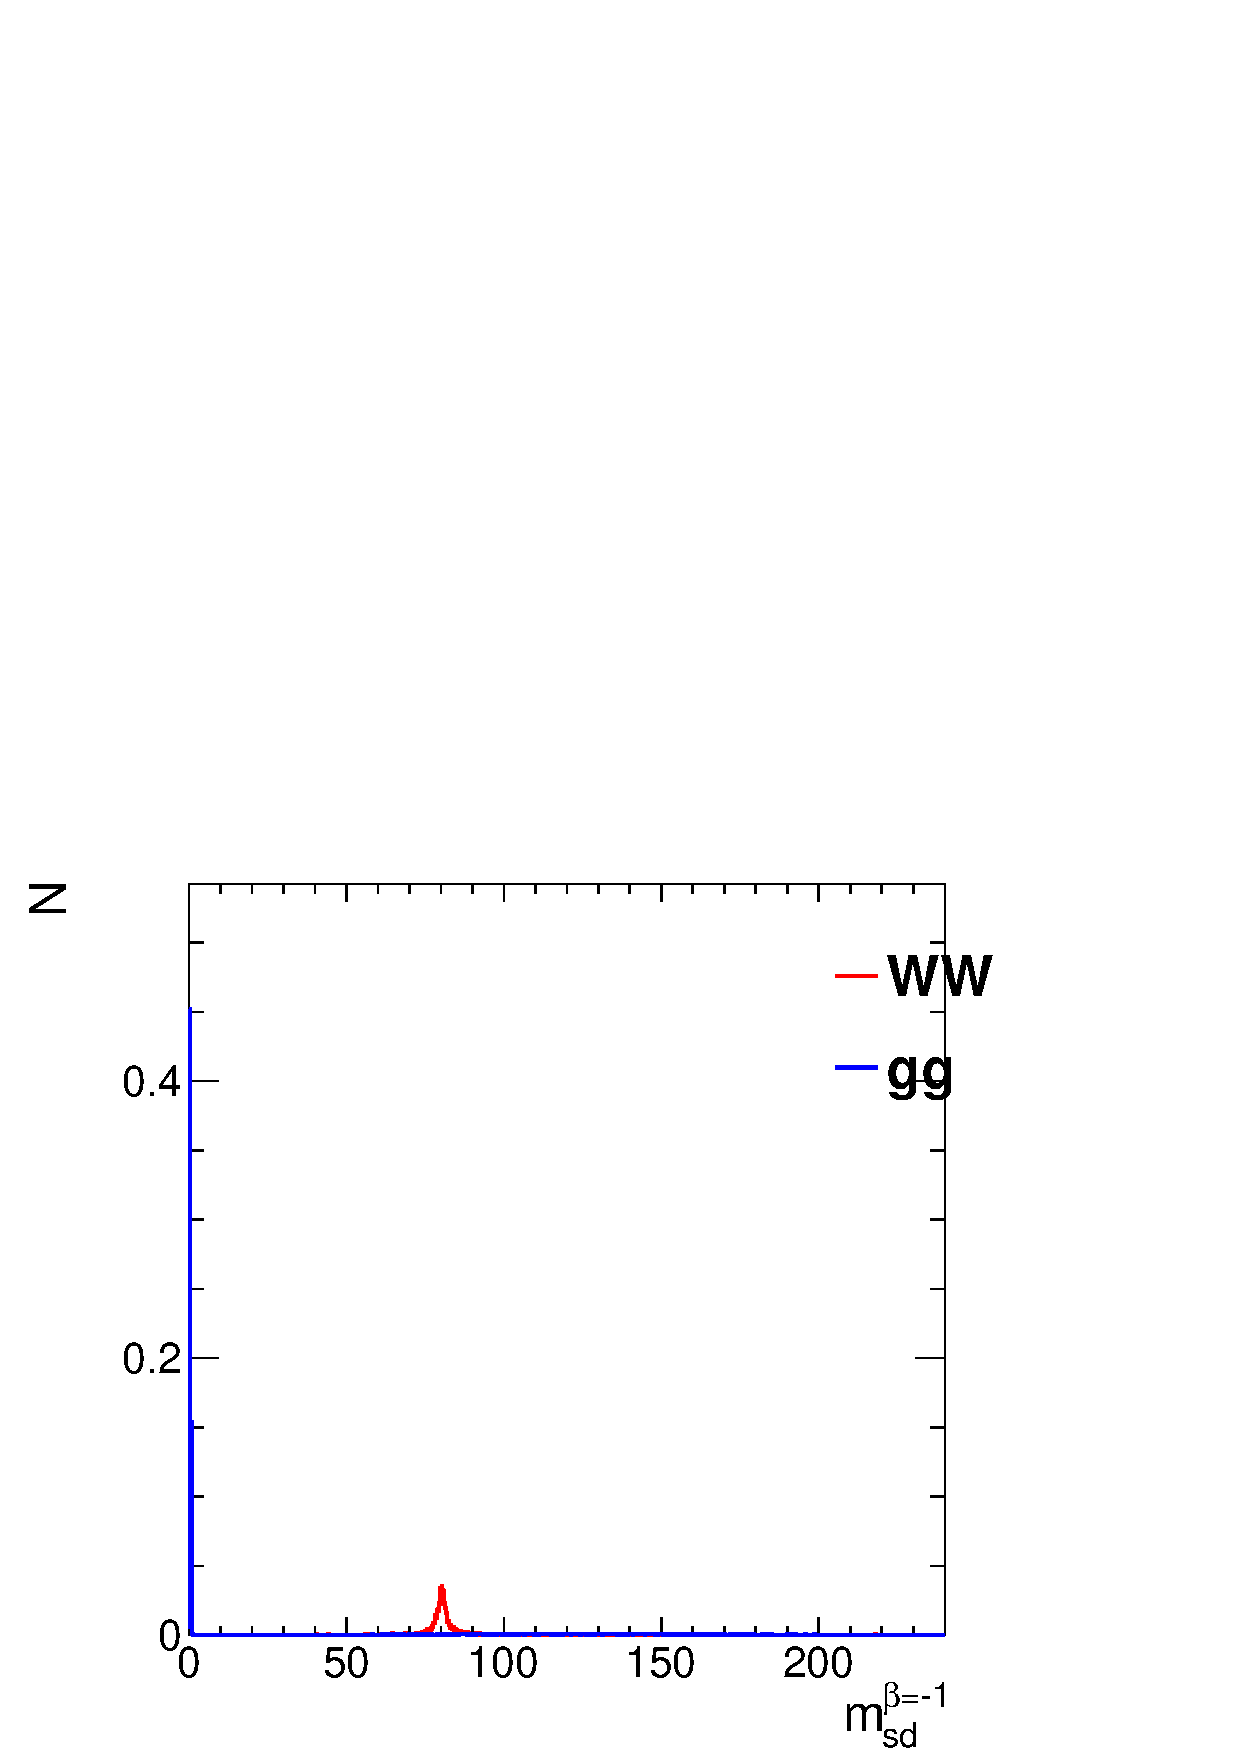
\includegraphics[width=0.30\textwidth]{./Figures/QGTagging/pT500/AKtR08/h_mass_sdm1.png}}
\caption{Comparisons of ungroomed and groomed quark and gluon mass distributions for leading jets in the 
$\pt=500-650 \GeV$ bin using the anti-\kT R=0.8 algorithm. }
\label{fig:qg_pt500_mass_AKt_R08}
\end{center}
\end{figure*}
Qualitatively, the application of grooming shifts the mass distributions towards
lower values as expected. No clear gain in discrimination can be seen, and for
certain grooming parameters, such as the use of soft drop with $\beta=-1$ a clear
loss in discrimination power is observed (\emph{BS: Is this just because the soft drop
kills off most of the radiation for both $q$/$g$ (the condition for $\beta=-1$ discards most of the collinear radiation)?}).
 Few variations are observed as the 
radius parameter of the jet reconstruction is increased in the two highest $\pt$ bins. 
However, for the $300-400\GeV$ bin, the use of small-$R$ jets produces a shift in the
mass distributions towards lower values, so that large-$R$ jet masses are more stable
with $\pt$ and small-$R$ jet masses are smaller at low-$\pt$ as expected from the spatial
constraints imposed by the $R$ parameter. These statements are explored more 
quantitatively later in this section. 

\begin{figure*}
\begin{center}
\subfigure[$C_1^{\beta=0}$]{\includegraphics[width=0.30\textwidth]{./Figures/QGTagging/pT500/AKtR08/h_c1_b0.png}}
\subfigure[$C_1^{\beta=1}$]{\includegraphics[width=0.30\textwidth]{./Figures/QGTagging/pT500/AKtR08/h_c1_b1.png}}
\subfigure[$C_1^{\beta=2}$]{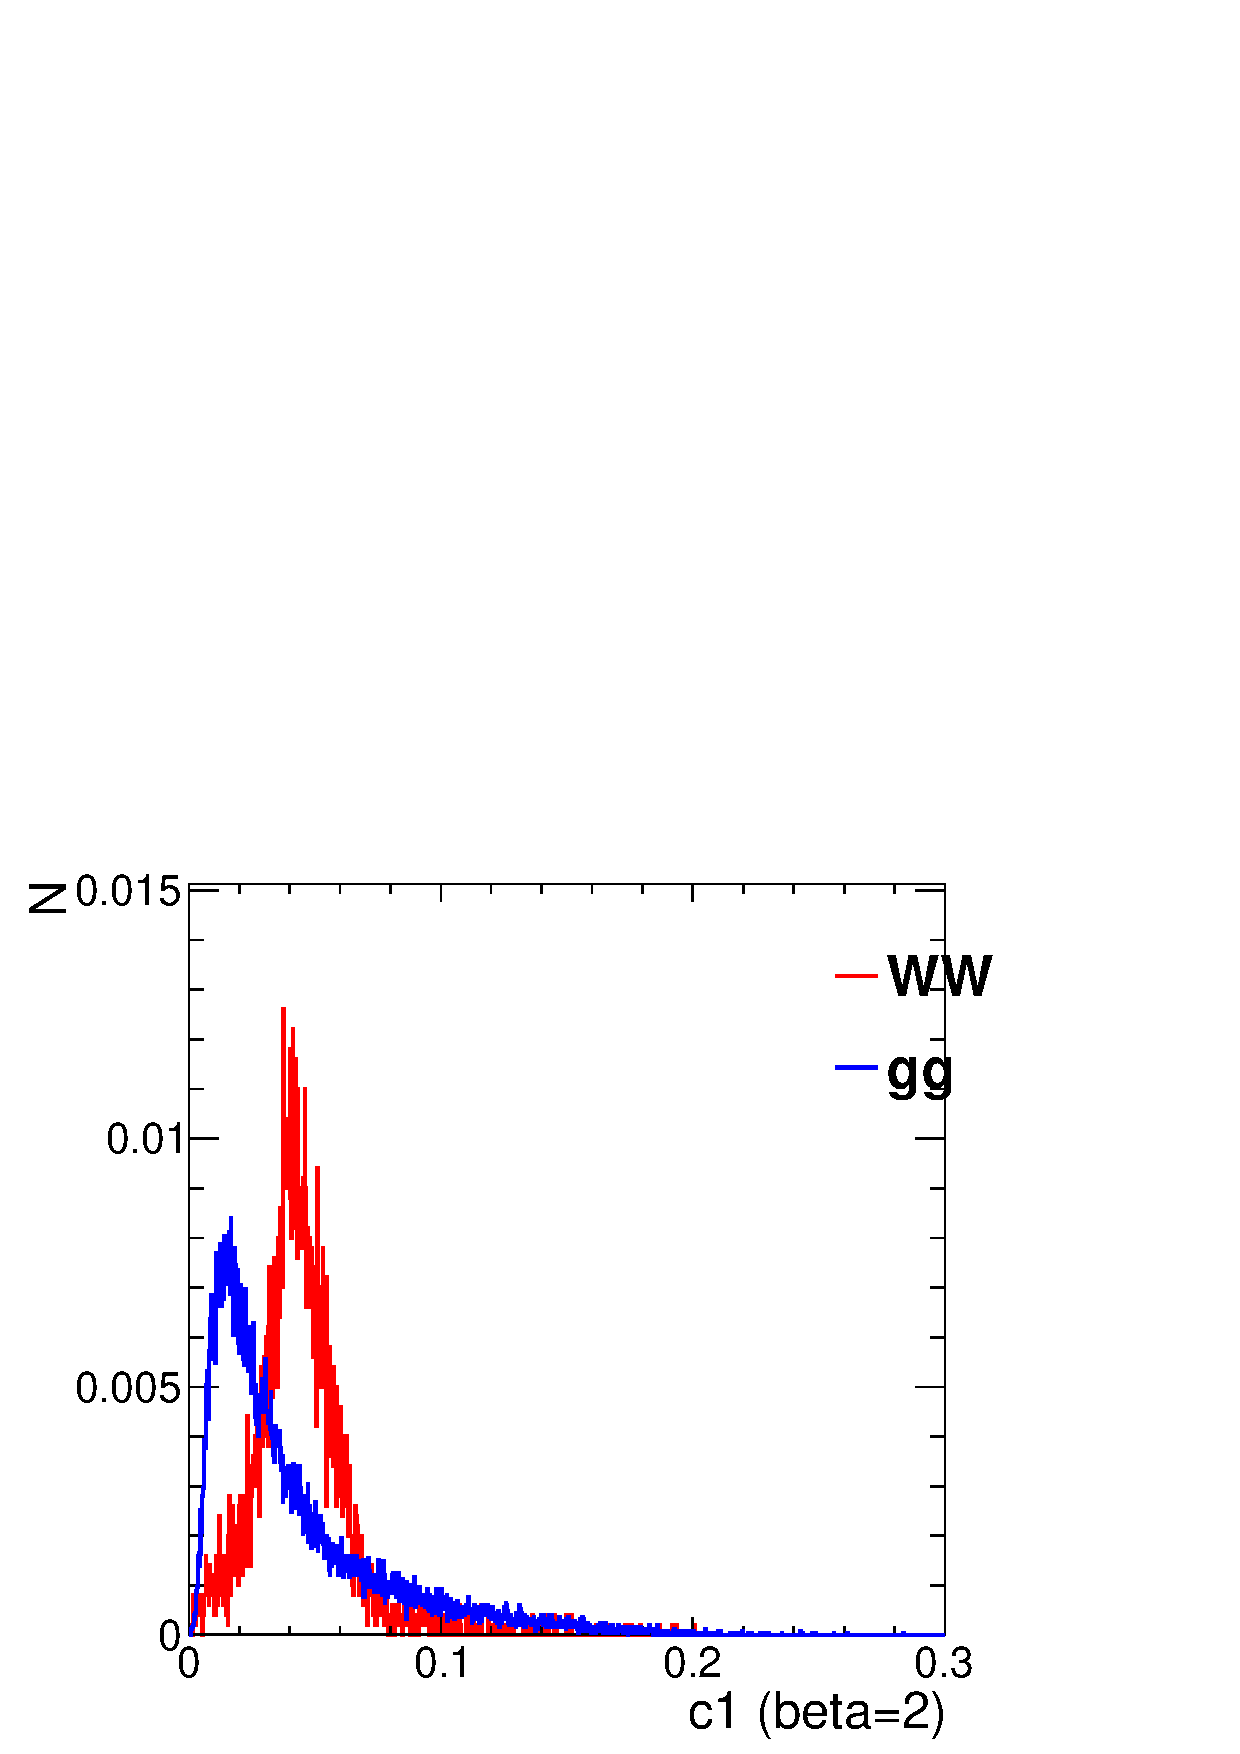
\includegraphics[width=0.30\textwidth]{./Figures/QGTagging/pT500/AKtR08/h_c1_b2.png}}\\
\subfigure[$\Gamma_{Qjet}$]{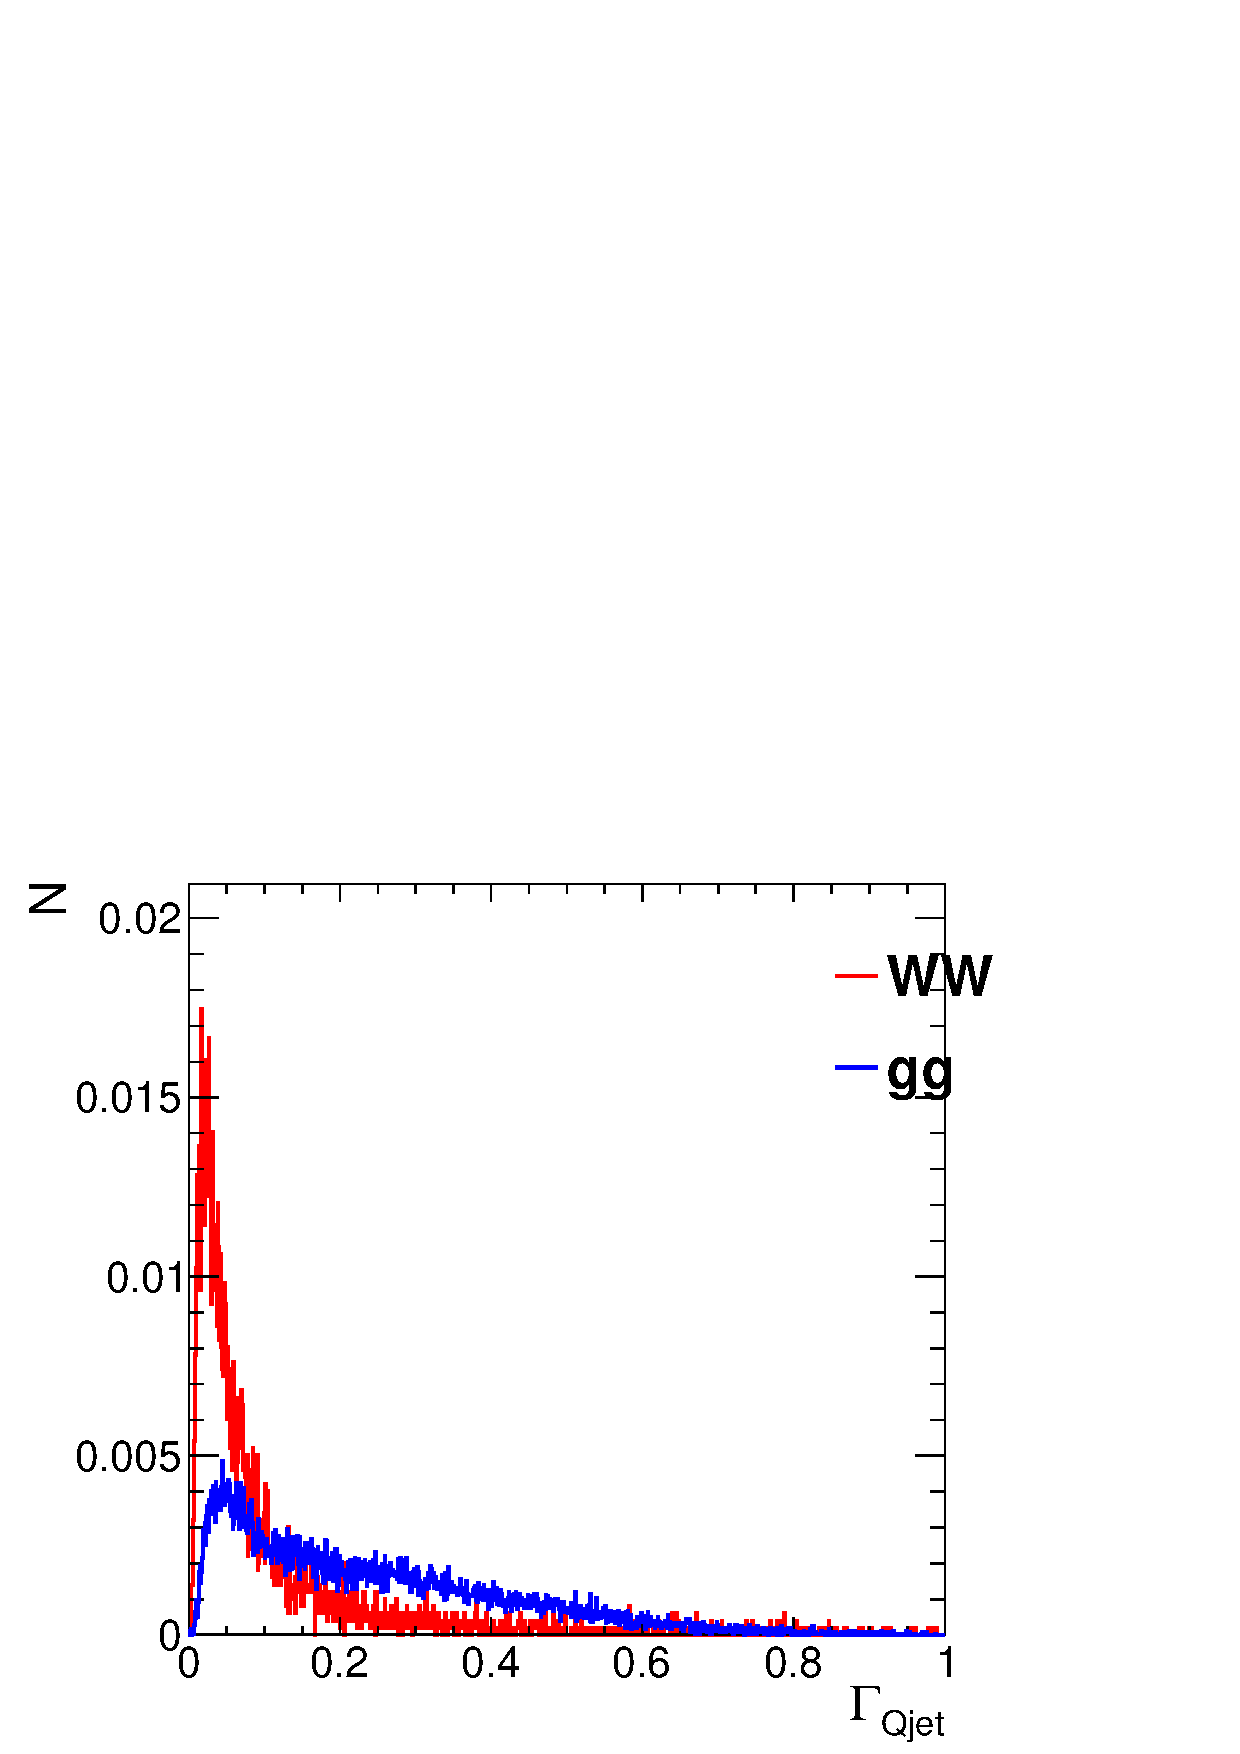
\includegraphics[width=0.30\textwidth]{./Figures/QGTagging/pT500/AKtR08/h_qjetVol.png}}
\subfigure[$\rm{n_ {constits}}$]{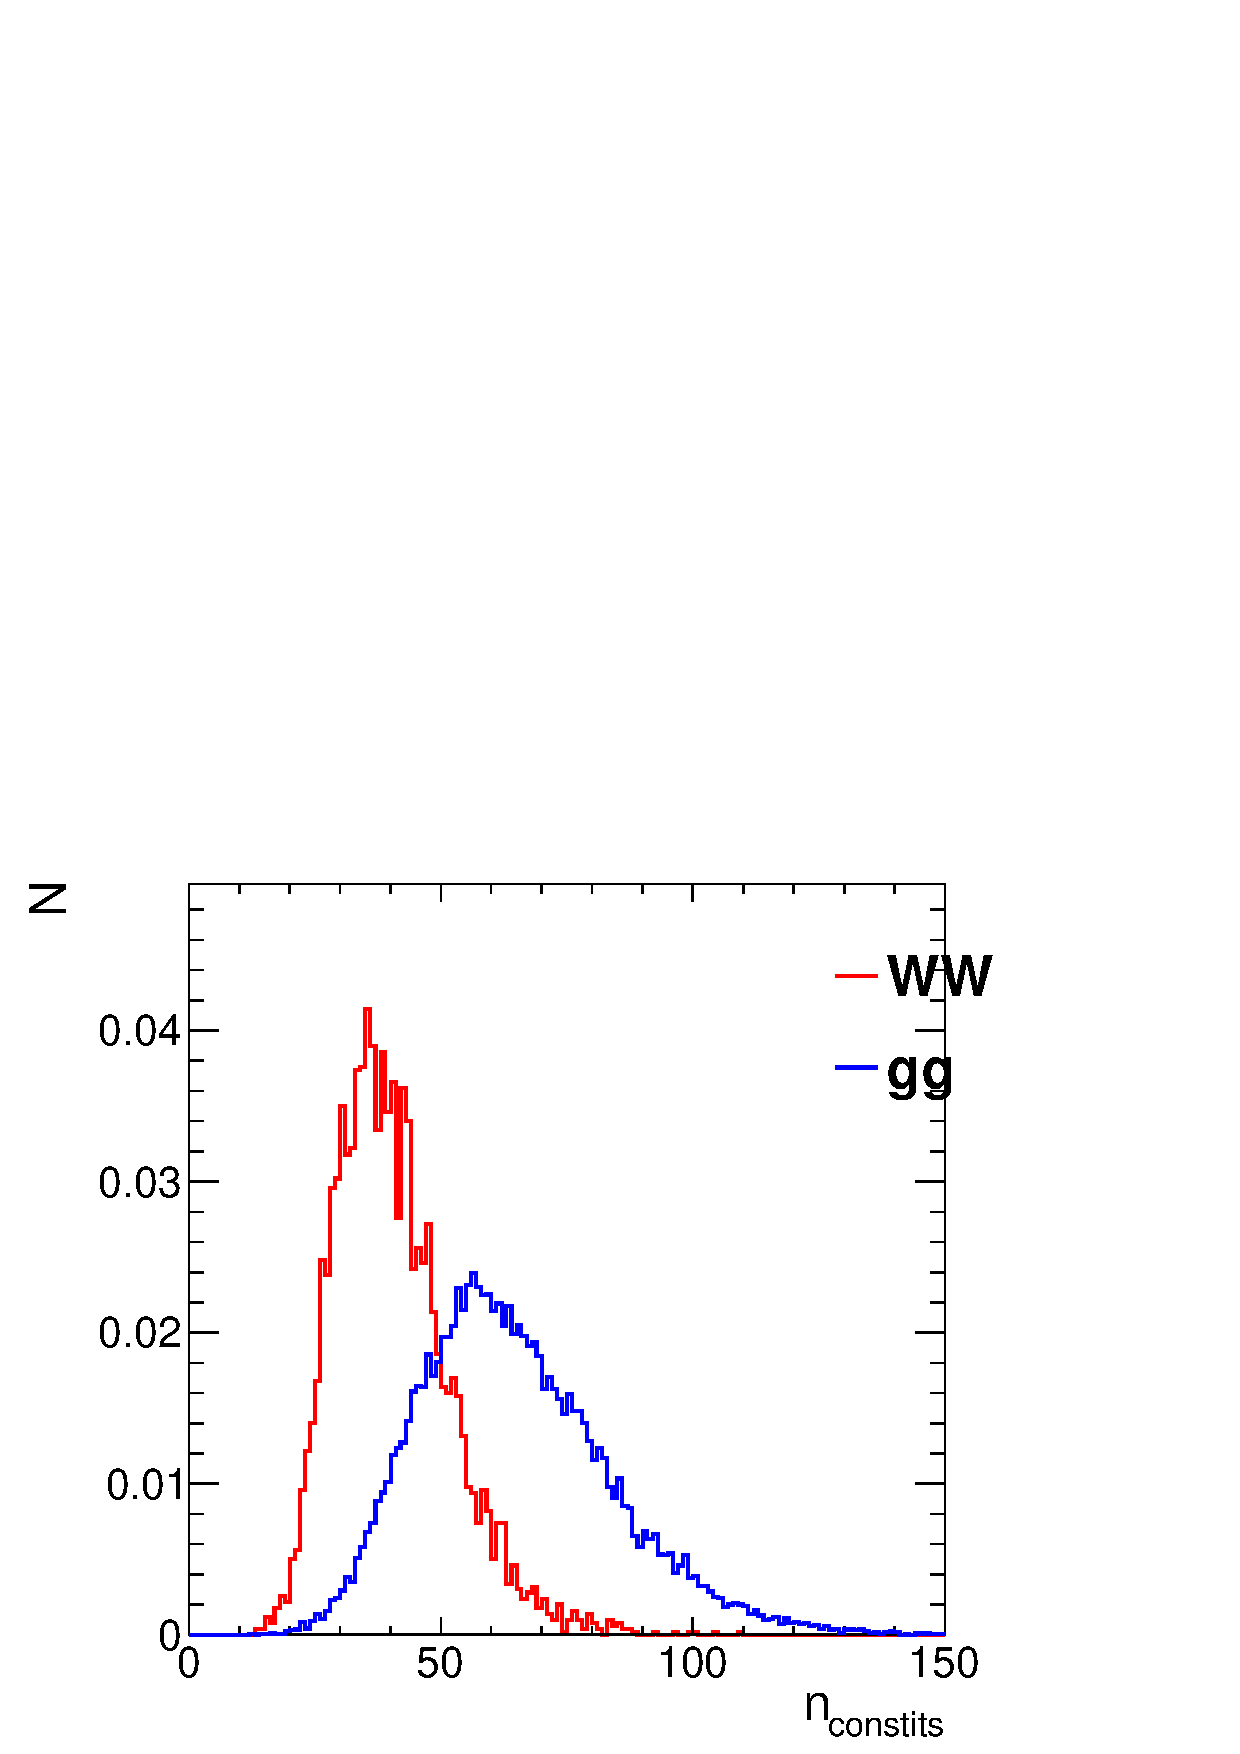
\includegraphics[width=0.30\textwidth]{./Figures/QGTagging/pT500/AKtR08/h_multiplicity.png}}
\subfigure[$\tau_{1}^{\beta=1}$]{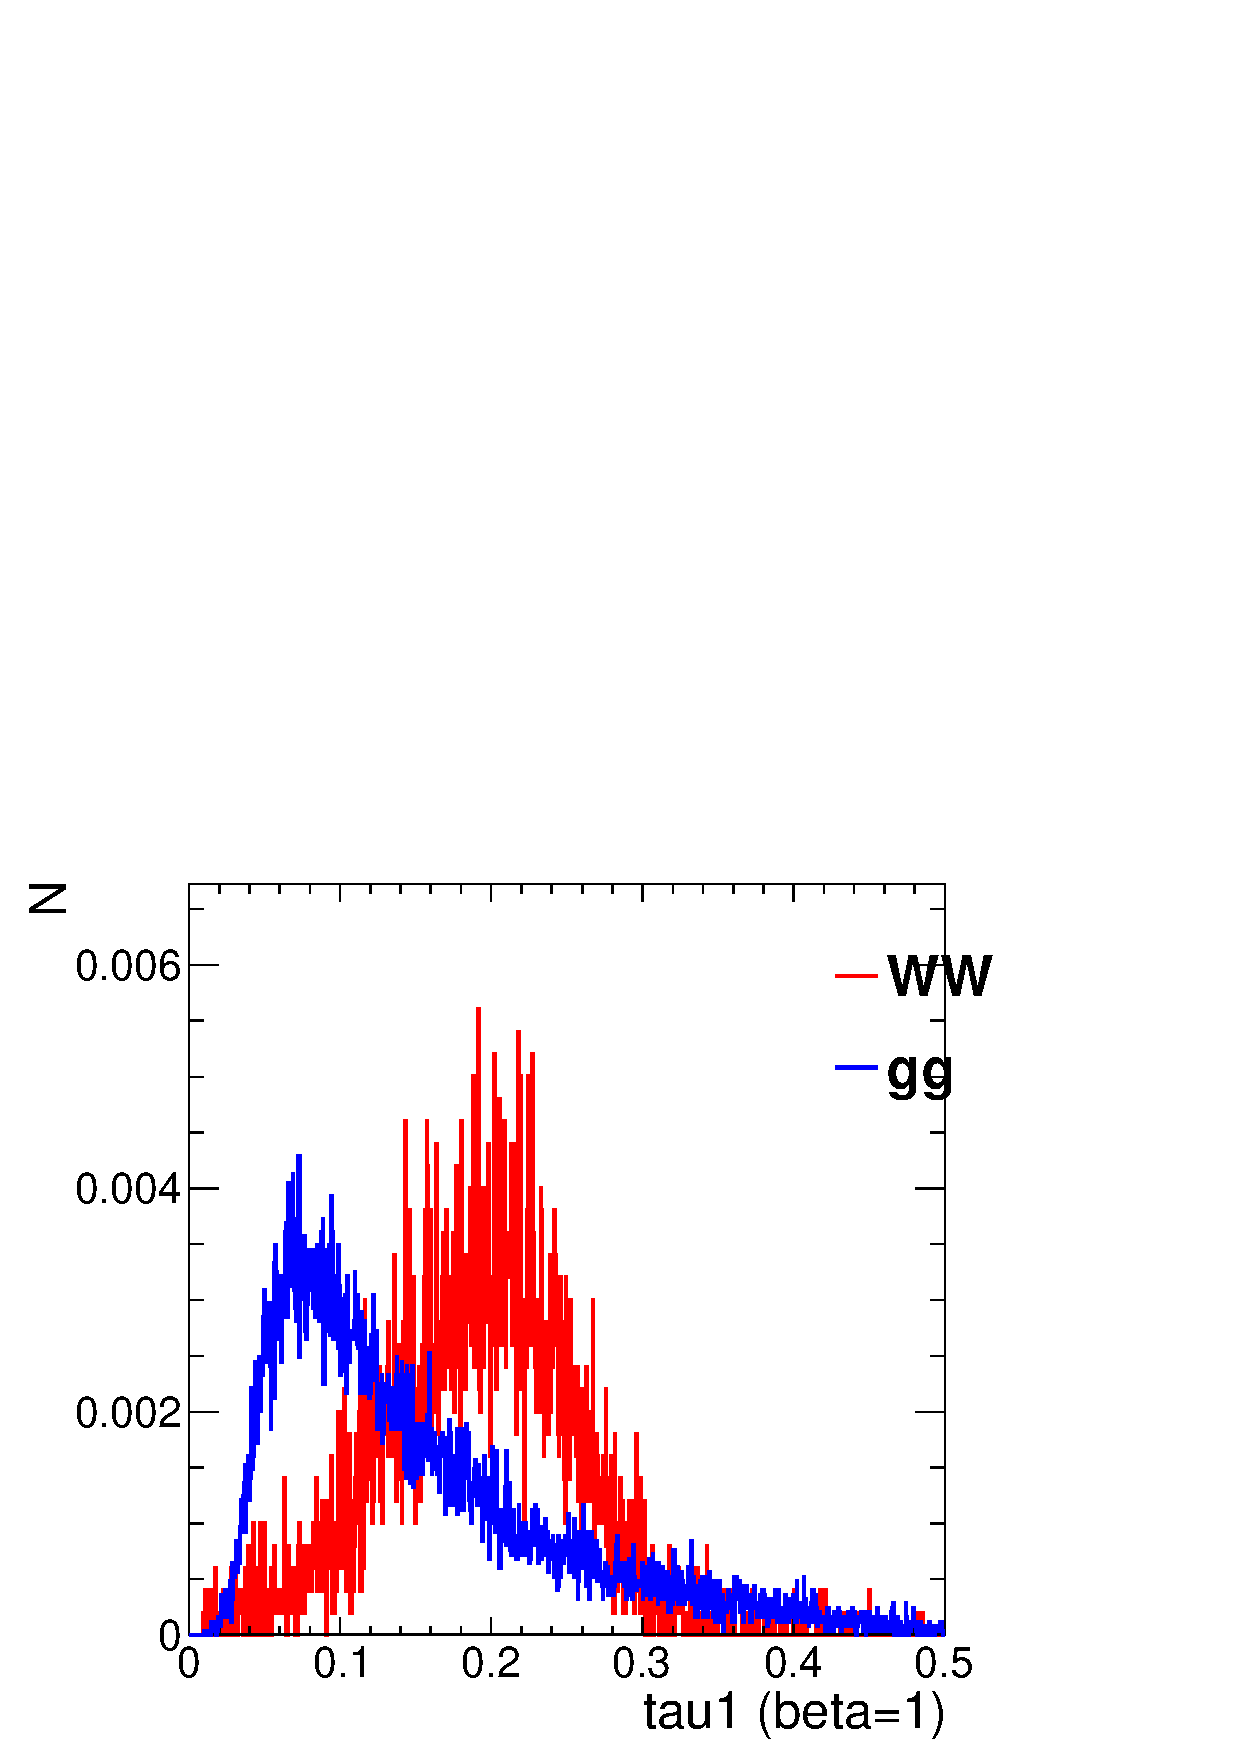
\includegraphics[width=0.30\textwidth]{./Figures/QGTagging/pT500/AKtR08/h_tau1_b1.png}}\\
\subfigure[$\tau_{1}^{\beta=2}$]{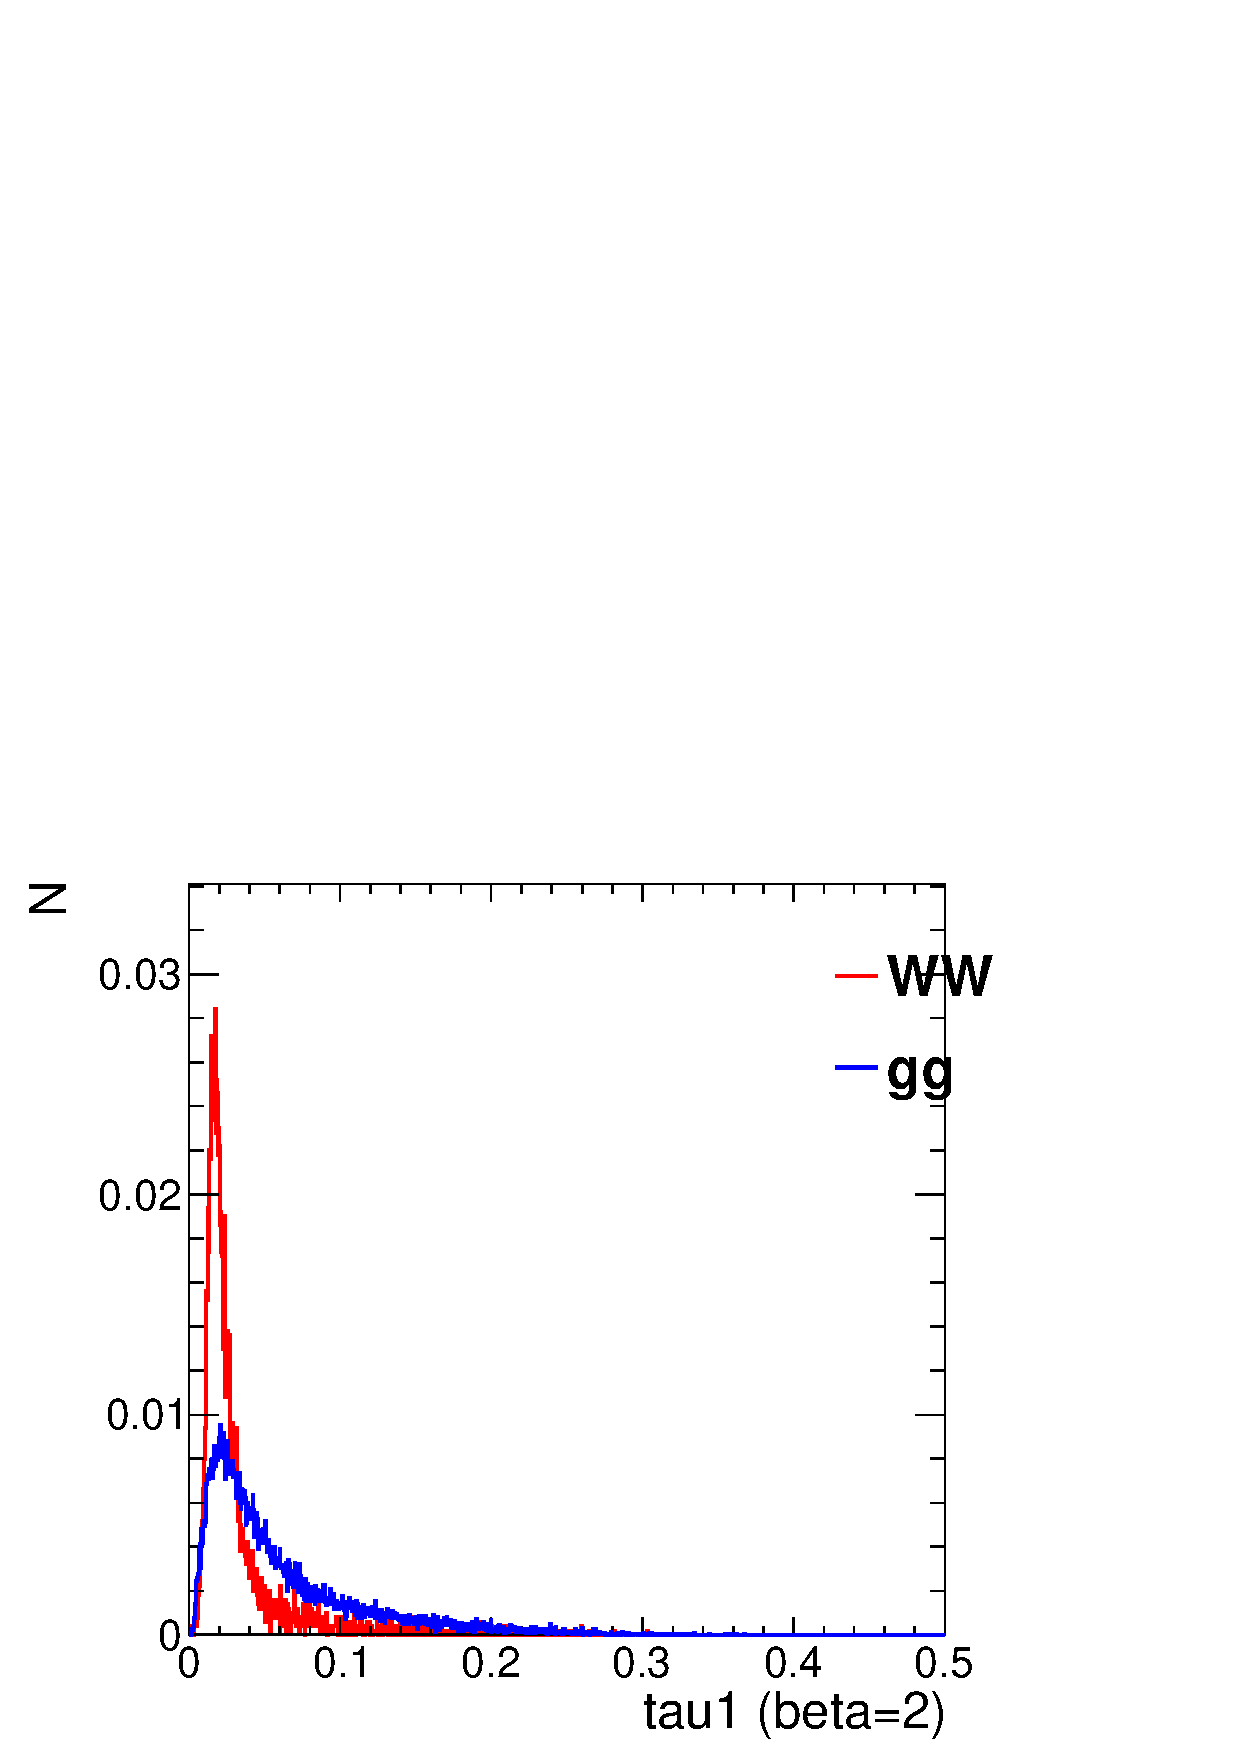
\includegraphics[width=0.30\textwidth]{./Figures/QGTagging/pT500/AKtR08/h_tau1_b2.png}}
\caption{Comparisons of quark and gluon distributions of different substructure variables for leading jets in the 
$\pt=500-650 \GeV$ bin using the anti-\kT R=0.8 algorithm. }
\label{fig:qg_pt500_subst_AKt_R08}
\end{center}
\end{figure*}

Among the different substructure variables explored, $n_{\rm constits}$ provides the highest separation
power, followed by $C_1^{\beta=0}$ and $C_1^{\beta=1}$ as was also found by the CMS and ATLAS Collaborations 
{\bf [add citations]}. The evolution of some of these distributions with $\pt$ and R is less trivial than
 for the jet masses. In particular, changing the R parameter at high $\pt$ changes significantly the $C_a^{\beta}$
for $\beta>0$ and the $n_{\rm constits}$ distributions, while leaving all other distributions qualitatively unchanged. 
This is illustrated in Figure~\ref{fig:Rdep_qg_C_pt1000} for $\beta=0$ and $\beta=1$ using $a=1$ in both cases for
jets with $\pt=1-1.2\TeV$. 
\begin{figure*}
\begin{center}
\subfigure[$C_1^{\beta=0}$, $R=0.4$]{\includegraphics[width=0.30\textwidth]{./Figures/QGTagging/pT1000/AKtR04/h_c1_b0.png}}
\subfigure[$C_1^{\beta=0}$, $R=0.8$]{\includegraphics[width=0.30\textwidth]{./Figures/QGTagging/pT1000/AKtR08/h_c1_b0.png}}
\subfigure[$C_1^{\beta=0}$, $R=1.2$]{\includegraphics[width=0.30\textwidth]{./Figures/QGTagging/pT1000/AKtR12/h_c1_b0.png}}\\
\subfigure[$C_1^{\beta=1}$, $R=0.4$]{\includegraphics[width=0.30\textwidth]{./Figures/QGTagging/pT1000/AKtR04/h_c1_b1.png}}
\subfigure[$C_1^{\beta=1}$, $R=0.8$]{\includegraphics[width=0.30\textwidth]{./Figures/QGTagging/pT1000/AKtR08/h_c1_b1.png}}
\subfigure[$C_1^{\beta=1}$, $R=1.2$]{\includegraphics[width=0.30\textwidth]{./Figures/QGTagging/pT1000/AKtR12/h_c1_b1.png}}\\
\caption{Comparisons of quark and gluon distributions of $C_1^{\beta=0}$ (top) and $C_1^{\beta=1}$ (bottom) 
for leading jets in the $\pt=1-1.2 \TeV$ bin using the anti-\kT algorithm with R=0.4,0.8 and 1.2. }
\label{fig:Rdep_qg_C_pt1000}
\end{center}
\end{figure*}
The shift towards lower values with changing R is evident for the $C_1^{\beta=1}$ distributions, while the stability
of $C_1^{\beta=0}$ can also be observed. These features are present in all $\pt$ bins studied, but are even more
pronounced for lower $\pt$ bins. The shape of the Q-jet volatility distribution shows some non-trivial shape that
deserves some explanation. Two peaks are observed, one at low volatility values and one at mid-volatility. These
peaks are generated by two somewhat distinct populations. The high volatility peak arises from jets that get their
mass primarily from soft (and sometimes wide-angle) emissions. The removal of some of the constituents when
building Q-jets thus changes the mass significantly, increasing the volatility. The lower volatility peak corresponds
to jets for which mass is generated by a hard emission, which makes the fraction of Q-jets that change 
the mass significantly to be smaller. Since the Sudakov form factors are larger for gluon jets, the low-volatility 
peak is higher for gluon jets by about the color factor $C_A/C_F$. 

To more quantitatively study the power of each observable as a
discriminator for quark/gluon tagging, Receiver Operating Characteristic (ROC) curves are built by scanning each distribution
and plotting the background efficiency (to select gluon jets) vs.~the signal efficiency (to select quark jets). 
Figure~\ref{fig:qg_pt300_single} shows these ROC curves for all of the variables shown in 
Figure~\ref{fig:qg_pt500_subst_AKt_R08} and the ungroomed mass, representing the 
best performing mass variable, for jets of $\pt=300-400\GeV$. In addition, the ROC curve for 
the tagger built from a BDT combining all the variables. The details of how the BDT is constructed 
are explained in Section~\ref{sec:multivariate}. 

\begin{figure*}
\begin{center}
\includegraphics[width=0.32\textwidth]{./Figures/QGTagging/pT300/AKtR04/Rocs_1D_single.png}
%\includegraphics[width=0.4\textwidth]{./Figures/QGTagging/pT1000/AKtR04/Rocs_1D_single.png}\\
\includegraphics[width=0.32\textwidth]{./Figures/QGTagging/pT300/AKtR08/Rocs_1D_single.png}
%\includegraphics[width=0.4\textwidth]{./Figures/QGTagging/pT1000/AKtR08/Rocs_1D_single.png}\\
\includegraphics[width=0.32\textwidth]{./Figures/QGTagging/pT300/AKtR12/Rocs_1D_single.png}
%\includegraphics[width=0.4\textwidth]{./Figures/QGTagging/pT1000/AKtR12/Rocs_1D_single.png}\\
\caption{The ROC curve for all single variables considered for quark-gluon discrimination in the \pt 500 GeV bin using the anti-\kT R=0.8 algorithm.}
\label{fig:qg_pt300_single}
\end{center}
\end{figure*}
Clearly, $n_{\rm constits}$ is the best performing variable for all Rs, even though $C_1^{\beta=0}$ is close, particularly
for R=0.8. Most other variables have similar performance, except the Q-jet volatility, which shows significantly worse
discrimination. The combination of all variables shows somewhat better discrimination. The overall discriminating 
power decreases with increasing R (\emph{BS: Do we understand if this is due to increased contamination from UE,
or if this is an actual physical effect?}), and the features discussed for this $\pt$ bin also apply to the higher
$\pt$ bins. This statement is quantified in the next section. 


\subsection{Correlations and Combined Performance}\label{sec:qg_combi}
The combined performance displayed in Fig.~\ref{fig:qg_pt300_single} is not much
better than that of single variables. However, that improvement in performance can
be critical for certain analyses requiring a quark/gluon tagger, and potentially larger in
data than in Monte Carlo simulation. Furthermore, insight can be gained into the 
features allowing for quark/gluon discrimination if how that improvement arises is
understood. It is therefore worth investigating quantitatively
the improvements in performance: to do so, quark/gluon taggers are built from
every pair-wise combination of variables studied in the previous section, as well as
the full set of variables using a boosted decision tree. 

In order to quantitatively study the value of each variable for quark/gluon tagging, the gluon 
rejection, defined as $1/\epsilon_{\rm gluon}$, is studied at a fixed quark selection efficiency
of 50\%. Figure~\ref{fig:qg_pt1000_comb} shows the rejection for each individual variable
(along the diagonal of the plots) and for each pair-wise combination. The rejection for the 
BDT combining all variables is also shown on the bottom right of each plot. Results are shown
for jets with $\pt=1-1.2 \TeV$ and for different $R$ parameters.
\begin{figure*}
\begin{center}
\includegraphics[width=0.32\textwidth]{./Figures/QGTagging/pT1000/AKtR04/effBkg2D.png}
%\includegraphics[width=0.4\textwidth]{./Figures/QGTagging/pT1000/AKtR04/Rocs_1D_single.png}\\
\includegraphics[width=0.32\textwidth]{./Figures/QGTagging/pT1000/AKtR08/effBkg2D.png}
%\includegraphics[width=0.4\textwidth]{./Figures/QGTagging/pT1000/AKtR08/Rocs_1D_single.png}\\
\includegraphics[width=0.32\textwidth]{./Figures/QGTagging/pT1000/AKtR12/effBkg2D.png}
%\includegraphics[width=0.4\textwidth]{./Figures/QGTagging/pT1000/AKtR12/Rocs_1D_single.png}\\
\caption{Gluon rejection defined as $1/\epsilon_{\rm gluon}$ when using each 2-variable combination 
as a tagger with 50\% acceptance for quark jets. Results are shown for jets with $\pt=1-1.2 \TeV$ and
for different $R$ parameters. The rejection obtained with a tagger that uses all variables is also shown
in the plots. }
\label{fig:qg_pt1000_comb}
\end{center}
\end{figure*}
As already observed in the previous section, $n_{\rm constits}$ is the most powerful single variable and
$\C{1}{\beta=0}$ follows closely. The combination of the two variables is also one of the most powerful
combinations for the two large-$R$ collections. Performance is generally better at small $R$, and in this case other pair-wise combinations are more powerful. In particular,
the combinations of $\tau^{\beta=1}_1$ or $\C{1}{\beta=1}$ with $n_{\rm constits}$ are capable of 
getting very  close to the rejection achievable through the use of all variables.

The overall loss in performance
with increasing $R$ can be observed in all single variables studied, except for $\C{1}{\beta=0}$ and 
the Q-jet volatility, which are quite resilient to increasing $R$. This is expected, since their distributions
were observed to be also quite insensitive to $R$ in the previous section. Their combination, however, does lose
performance significantly as R is increased. {\bf [do we understand this?]}
Of all the variables studied, $\beta=2$ 1-subjettiness and energy correlation variables 
are particularly sensitive to increasing R. This is understandable, because for $\beta=2$ 
a larger weight is put in large-angle emissions. However, from other variables, it is understood
that most of the discrimination power comes from analyzing a small-R jet, or the center of the
large-R jet. 

These observations are qualitatively similar across all ranges of $\pt$. Quantitatively, however,
there is a loss of rejection power for the taggers made of a combination of variables as the $\pt$ decreases. 
This can be observed in Fig.~\ref{fig:qg_akt4_comb} for anti-$\kT$ R=0.4 jets of different $\pt$s. 
\begin{figure*}
\begin{center}
\includegraphics[width=0.32\textwidth]{./Figures/QGTagging/pT300/AKtR04/effBkg2D.png}
%\includegraphics[width=0.4\textwidth]{./Figures/QGTagging/pT1000/AKtR04/Rocs_1D_single.png}\\
\includegraphics[width=0.32\textwidth]{./Figures/QGTagging/pT500/AKtR04/effBkg2D.png}
%\includegraphics[width=0.4\textwidth]{./Figures/QGTagging/pT1000/AKtR08/Rocs_1D_single.png}\\
\includegraphics[width=0.32\textwidth]{./Figures/QGTagging/pT1000/AKtR04/effBkg2D.png}
%\includegraphics[width=0.4\textwidth]{./Figures/QGTagging/pT1000/AKtR12/Rocs_1D_single.png}\\
\caption{Gluon rejection defined as $1/\epsilon_{\rm gluon}$ when using each 2-variable combination 
as a tagger with 50\% acceptance for quark jets. Results are shown for R=0.4 jets with $\pt=300-400 \GeV$, 
$\pt=500-600 \GeV$ and $\pt=1-1.2 \TeV$. The rejection obtained with a tagger that uses all variables is also shown
in the plots. }
\label{fig:qg_akt4_comb}
\end{center}
\end{figure*}
Clearly, most single variables retain their gluon rejection potential at lower $\pt$s. However, when combined
with other variables, the highest performing pairwise combinations lose ground with respect to other pairwise 
combinations. This is also reflected in the rejection of the tagger that uses a combination of all variables, which
is lower at lower $\pt$s. {\bf [do we understand this?]}

(\emph{BS: Do we want to explicitly mention some aspects of the correlation, namely quantifying which observables seem to be most correlated and that it seems that the all-variable performance is not much better than some of the pair-wise combinations, and so there seem to be $\sim2$ independent observables? Also, I remember Nhan had some tables that showed some variable rankings in terms of how (un)correlated they were; not sure if we want to show these.}

%\subsection{QJets Volatility and $\ptd$ ($\C{1}{\beta=0}$)}

%Simple explanation of correlation, or why does combining volatility and $\ptd$ improve quark versus gluon discrimination.  $\ptd$ ($\C{1}{\beta=0}$) takes small (large) values for a jet with near-democratic energy sharing between particles and large (small) values when the energy of the jet is contained in a few particles.  Because we expect gluons to radiate more particles, we expect that $\ptd_g<\ptd_q$ (or ${\C{1}{\beta=0}}_g>{\C{1}{\beta=0}}_q$).  Now, we expect the volatility of gluon jets to be in general smaller than that of quark jets because there is a greater probability (by a factor of about $C_A/C_F=9/4$) that there was a relatively hard emission in a jet that is not groomed away.  By measuring both volatility and $\ptd$, we are sensitive to both regions of phase space: where a relatively hard emission dominates the mass of the jet as well as the region where many soft emissions set the jet mass.
